%% paper.tex — шаблон статьи учебной конференции AI4Science-YSDA 2026
%%
%% Сборка:
%%     pdflatex paper
%%     bibtex   paper
%%     pdflatex paper
%%     pdflatex paper
%%
%% ВЕРСИИ. Сведения об авторах заполняются сразу. Что из них печатается,
%% задаёт опция пакета ai4science_ysda2026:
%%     без опций   обезличенная версия для подачи: вместо авторов печатается
%%                 «Анонимные авторы», организации, адрес почты и благодарности
%%                 скрыты, поле автора в метаданных PDF пустое, слева стоят
%%                 номера строк для рецензента
%%     final       итоговая версия после рецензирования
%%     english     статья на английском языке: [english] или [english,final]
%%
%% ОБЪЁМ. От двух до четырёх страниц основного текста. Список литературы,
%% раздел «Использование ИИ-ассистентов» и приложения в объём не входят.
%% Поля, шрифт и интервалы не меняются.
%%
%% ПОМЕТКИ АВТОРСТВА
%%     \porozhdeno{...}  фрагмент порождён моделью           [порождено]
%%     \napisano{...}    фрагмент написан автором            [написано]
%%     \istochnik{...}   фрагмент взят из источника          [источник]
%% Необязательный аргумент уточняет пометку: \porozhdeno[модель, версия]{...}.
%% С пустыми фигурными скобками печатается только пометка: \porozhdeno{}.
%% В статье на английском языке: \generated, \written, \sourced.
%%
%% ОБЕЗЛИЧИВАНИЕ
%%     \anonymized{...}        в обезличенной версии вместо текста печатается
%%                             «[скрыто на время рецензирования]»
%%     \finalonly{...}         текст печатается только в итоговой версии
%%     \acknowledgements{...}  раздел «Благодарности», только в итоговой версии
%% В тексте, в подписях, в именах файлов и в приложенном архиве нет имён,
%% адресов почты и ссылок на личные страницы и репозитории. На свои прошлые
%% работы ссылаются в третьем лице.

\documentclass{article}

\usepackage{ai4science_ysda2026}            % обезличенная версия для подачи
% \usepackage[final]{ai4science_ysda2026}   % итоговая версия

\usepackage{amsmath}
\usepackage{amssymb}
\usepackage{amsthm}
\usepackage{graphicx}
\usepackage{booktabs}
\usepackage{microtype}
% здесь подключаются нужные авторам пакеты

\theoremstyle{plain}
\newtheorem{theorem}{Теорема}
\newtheorem{lemma}[theorem]{Лемма}
\newtheorem{proposition}[theorem]{Предложение}
\theoremstyle{definition}
\newtheorem{definition}[theorem]{Определение}

% Короткое название печатается в колонтитуле со второй страницы
\icmltitlerunning{Короткое название статьи}

\begin{document}

\twocolumn[
  \icmltitle{Название статьи}

  \begin{icmlauthorlist}
    \icmlauthor{И.~И.~Иванов}{org1}
    \icmlauthor{П.~П.~Петров}{org1,org2}
  \end{icmlauthorlist}

  \icmlaffiliation{org1}{Организация, город, страна}
  \icmlaffiliation{org2}{Организация, город, страна}

  \icmlcorrespondingauthor{И.~И.~Иванов}{author@example.org}

  \icmlkeywords{словосочетание 1, словосочетание 2, словосочетание 3}

  \vskip 0.3in
]

% сноска первой страницы: организации и адрес почты (в итоговой версии),
% строка о конференции
\printAffiliationsAndNotice{}

\begin{abstract}
Краткое изложение работы: задача и её место в своей области, метод, способ
проверки и главный результат с числом и мерой разброса. В аннотации
не используются формулы, ссылки на литературу и сокращения без расшифровки.
\end{abstract}

\section{Введение}
\label{sec:intro}

Назовите задачу и объясните, зачем она нужна в вашей области. Сформулируйте
вопрос исследования одной фразой и перечислите, что получено в работе: метод,
способ проверки, главный результат с числом.
\porozhdeno[модель, версия]{Предложение, порождённое моделью и проверенное
автором, остаётся в тексте с пометкой.}
\istochnik{Утверждение, взятое из чужой работы, получает пометку и
ссылку~\cite{roy2005}.}

Оформление разделов показано ниже на учебной задаче: проверка порядка
сходимости реализации численного метода.

\section{Постановка задачи}
\label{sec:problem}

Постановка отвечает на три вопроса: что дано, что требуется получить и по
какому критерию результат считается верным. Критерий записывается так, чтобы
его можно было проверить запуском программы или доказательством. Обозначения
вводятся один раз и не меняют смысла до конца статьи.

\textbf{Дано.} Задача Коши $y' = \lambda y$, $y(0) = 1$ на отрезке $[0, 1]$
с точным решением $y(t) = e^{\lambda t}$ и реализация одношагового метода
с заявленным порядком сходимости~$q$. Численное решение с шагом $h = 1/N$
даёт погрешность $e(h) = |y_N - y(1)|$.

\begin{definition}
Эмпирическим порядком сходимости по паре шагов $h$ и $h/2$ называется
величина
\begin{equation}\label{eq:order}
  p = \log_2 \frac{e(h)}{e(h/2)}.
\end{equation}
\end{definition}

\textbf{Требуется.} Установить, сходится ли реализация с заявленным
порядком~$q$.

\textbf{Критерий.} Реализация принимается, если $|p - q| \le 0{,}05$ для
каждого значения seed, и отклоняется в противном случае.

\section{Место в области}
\label{sec:related}

Опишите известные подходы к задаче со ссылками на
литературу~\cite{hairer1990, roy2005, sandve2013} и для каждой работы
скажите, чем от неё отличается ваша. В обезличенной версии на свои работы
ссылаются в третьем лице.

\section{Метод}
\label{sec:method}

Изложите метод так, чтобы его можно было повторить: модель, алгоритм, данные
и параметры. Утверждение формулируется вместе с условиями и сопровождается
доказательством или ссылкой на него. Нумеруются только формулы, на которые
есть ссылки.

\begin{proposition}\label{prop:order}
Если $e(h) = C h^{q} + O(h^{q+1})$ при $h \to 0$ и $C \neq 0$, то
$p = q + O(h)$.
\end{proposition}

\begin{proof}
Подставим разложение в~\eqref{eq:order}:
\[
  \frac{e(h)}{e(h/2)} = 2^{q}\,\bigl(1 + O(h)\bigr),
\]
откуда $p = q + \log_2\bigl(1 + O(h)\bigr) = q + O(h)$.
\end{proof}

Для явного метода Эйлера $q = 1$, для явного метода средней точки
$q = 2$~\cite{hairer1990}. По предложению~\ref{prop:order} величина $p$ при
малом шаге близка к $q$, если реализация верна.

\section{Проверка}
\label{sec:verification}

Опишите, что проверяется, каким верификатором, по какому критерию результат
принимается и какие ошибки проверка поймала. В учебной задаче верификатор
вычисляет $p$ по формуле~\eqref{eq:order} для $h = 2^{-9}$ и применяет
критерий раздела~\ref{sec:problem}. Внесённая ошибка (в шаге метода средней
точки приращение умножено на $h/2$ вместо $h$) даёт $p \approx 0$,
и верификатор отклоняет реализацию (табл.~\ref{tab:order}).

% Название таблицы стоит над ней. Ссылка на таблицу и на рисунок даётся
% в тексте до них. Числа таблицы берутся из файла результатов.
\begin{table}[t]
  \caption{Порядок сходимости $p$ по $r = 5$ значениям seed: среднее $\pm$
    стандартное отклонение.}
  \label{tab:order}
  \centering
  \small
  \setlength{\tabcolsep}{4.5pt}
  \begin{tabular}{@{}lccl@{}}
    \toprule
    Вариант                 & $q$ & $p$                     & Решение   \\
    \midrule
    Метод Эйлера            & 1   & $1{,}0006 \pm 0{,}0001$ & принято   \\
    Метод средней точки     & 2   & $2{,}0013 \pm 0{,}0005$ & принято   \\
    Средняя точка с ошибкой & 2   & $0{,}0006 \pm 0{,}0003$ & отклонено \\
    \bottomrule
  \end{tabular}
\end{table}

\section{Эксперимент}
\label{sec:experiment}

Приведите план эксперимента: что варьируется и что фиксируется, число значений
seed~$r$, метрику и меру разброса. Два варианта, разность метрик которых
сравнима с разбросом, сравниваются на общих значениях seed с указанием
статистического критерия и уровня значимости.

В учебной задаче seed задаёт коэффициент $\lambda$, равномерно распределённый
на отрезке от $-2$ до $-0{,}5$, число значений seed $r = 5$, шаги
$h = 2^{-k}$, $k = 4, \dots, 10$. Результаты приведены в
табл.~\ref{tab:order} и на рис.~\ref{fig:order}. Стандартное отклонение $p$
по значениям seed меньше $10^{-3}$ и много меньше допуска $0{,}05$, поэтому
решение верификатора устойчиво к выбору seed.

% Подпись стоит под рисунком. Рисунок подготовлен в ширину колонки (8,2 см)
% и вставляется без масштабирования, подписи осей читаются при печати.
\begin{figure}[t]
  \centering
  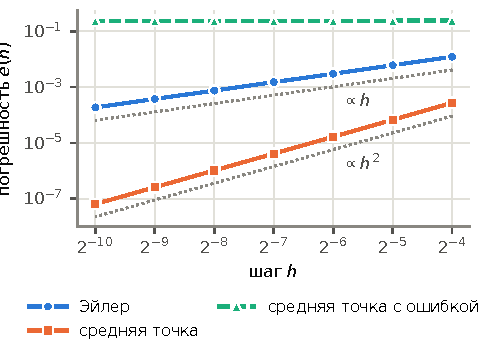
\includegraphics[width=\columnwidth]{figures/example_figure.pdf}
  \caption{Погрешность $e(h)$ для seed 0 ($\lambda \approx -1{,}04$).
    Точечные линии — зависимости $\propto h$ и $\propto h^{2}$.}
  \label{fig:order}
\end{figure}

\section{Ограничения}
\label{sec:limitations}

Перечислите условия, при которых результат может оказаться неверным или
не переносится на другие задачи: допущения модели, область применимости, объём
и происхождение данных, то, чего проверка не покрывает. В учебной задаче
проверка выполнена на одном линейном автономном уравнении, поэтому ошибки
в аргументе времени и ошибки, сохраняющие порядок метода, верификатор
не обнаружит.

\section{Воспроизводимость}
\label{sec:reproducibility}

Укажите, где лежат код и данные, метку git, по которой воспроизводится
результат, окружение и команду запуска. Ссылка на личный репозиторий
в обезличенной версии скрывается: \anonymized{\url{https://example.org/repo}},
к подаче прилагается обезличенный архив. Табл.~\ref{tab:order}
и рис.~\ref{fig:order} получены командой
\texttt{python figures/example\_figure.py} (Python~3.10, numpy~1.26,
matplotlib~3.9).

\section{Заключение}
\label{sec:conclusion}

Кратко повторите главный результат с числом и мерой разброса, назовите
основные ограничения и следующий шаг работы.

\begin{aiusage}[Укажите фрагменты, порождённые моделью или взятые из
  источников, и способ их проверки.]
  Введение, абзац 1 & \porozhdeno{} & модель, версия
    & сверено с постановкой задачи \\
  Код верификатора & \porozhdeno{} & агент, модель
    & прогон на методах с известным порядком (табл.~\ref{tab:order}) \\
  Раздел~\ref{sec:related} & \istochnik{} & поиск по библиотеке
    & утверждения сверены с работами~\cite{hairer1990, roy2005} \\
  Остальной текст & \napisano{} & --- & --- \\
\end{aiusage}

\acknowledgements{Авторы благодарят \ldots}

\bibliography{paper}
\bibliographystyle{ai4science_ysda2026}

% Приложения необязательны, идут после списка литературы и не входят в объём
% статьи: состав архива с кодом и данными, команды запуска, доказательства
% и таблицы, без которых основной текст читается.
% \appendix
% \onecolumn
% \section{Код и данные}

\end{document}
